\documentclass[tikz,border=4mm]{standalone}
\usepackage{tikz}
\usetikzlibrary{arrows.meta, positioning, calc}
\usepackage{amsmath}
\usepackage{amssymb}

%% Palette – blue-grey, RA-L compatible, greyscale-friendly
\definecolor{clrA} {RGB}{219,232,244}  % light steel-blue  (data nodes)
\definecolor{clrB} {RGB}{149,196,234}  % medium steel-blue (model nodes)
\definecolor{clrC} {RGB}{ 31, 73,125}  % dark navy         (execute nodes)
\definecolor{clrBd}{RGB}{ 68,114,196}  % border / arrow colour
\definecolor{clrGr}{RGB}{ 89, 89, 89}  % annotation grey

\begin{document}
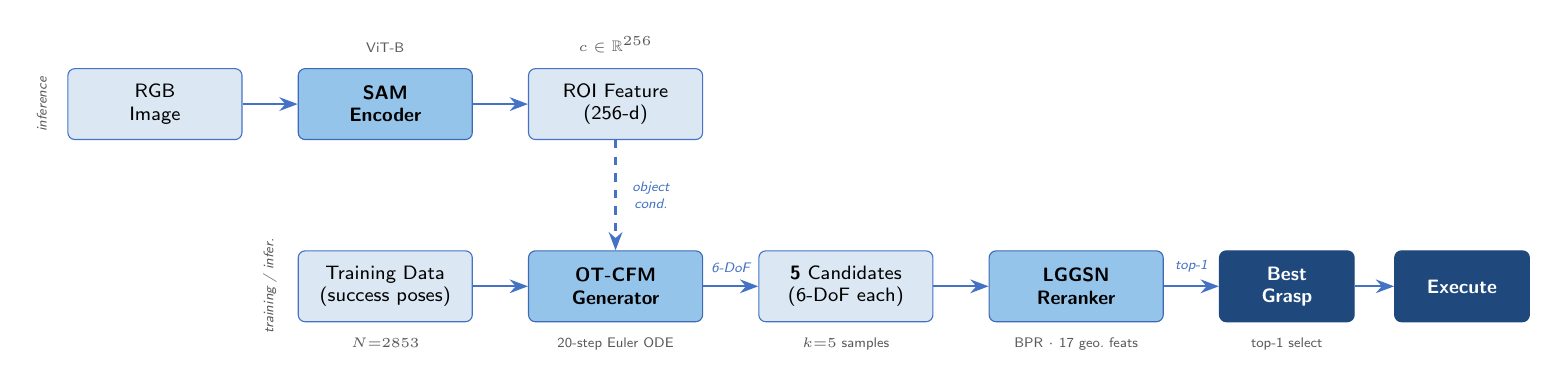
\begin{tikzpicture}[
  %% ── node styles ──────────────────────────────────────────────────────────
  dnode/.style = {rectangle, rounded corners=2.5pt,
                  minimum height=9mm, text width=20mm, align=center,
                  inner sep=3pt, draw=clrBd, fill=clrA,
                  font=\scriptsize\sffamily},
  mnode/.style = {rectangle, rounded corners=2.5pt,
                  minimum height=9mm, text width=20mm, align=center,
                  inner sep=3pt, draw=clrBd!80!clrC, fill=clrB,
                  font=\scriptsize\sffamily\bfseries},
  enode/.style = {rectangle, rounded corners=2.5pt,
                  minimum height=9mm, text width=15mm, align=center,
                  inner sep=3pt, draw=clrC, fill=clrC,
                  text=white, font=\scriptsize\sffamily\bfseries},
  %% ── arrow / label styles ─────────────────────────────────────────────────
  arr/.style  = {-Stealth, thick, color=clrBd},
  darr/.style = {-Stealth, thick, color=clrBd, dashed},
  ann/.style  = {font=\fontsize{5.5}{6.5}\selectfont\sffamily,
                 color=clrGr, align=center},
  lab/.style  = {font=\fontsize{5.5}{6.5}\selectfont\sffamily\itshape,
                 color=clrBd, align=center},
]

%% ═══════════════════════════════════════════════════════════════════════════
%% BOTTOM ROW  (y = 0): training data → generation → reranking → execution
%% ═══════════════════════════════════════════════════════════════════════════
\node[dnode] (data)  at (0,0)                    {Training Data\\(success poses)};
\node[mnode, right=7mm of data]  (cfm)            {OT-CFM\\Generator};
\node[dnode, right=7mm of cfm]   (cands)          {\textbf{5} Candidates\\(6-DoF each)};
\node[mnode, right=7mm of cands] (lggsn)          {LGGSN\\Reranker};
\node[enode, right=7mm of lggsn] (best)           {Best\\Grasp};
\node[enode, right=5mm of best]  (exec)           {Execute};

%% ═══════════════════════════════════════════════════════════════════════════
%% TOP ROW: feat directly above cfm, then sam and img to its left
%% ═══════════════════════════════════════════════════════════════════════════
\node[dnode, above=14mm of cfm]  (feat)  {ROI Feature\\(256-d)};
\node[mnode, left=7mm of feat]   (sam)   {SAM\\Encoder};
\node[dnode, left=7mm of sam]    (img)   {RGB\\Image};

%% ── top-row arrows ────────────────────────────────────────────────────────
\draw[arr] (img)  -- (sam);
\draw[arr] (sam)  -- (feat);

%% ── conditioning: straight vertical dashed arrow feat → cfm ──────────────
\draw[darr] (feat.south) -- (cfm.north);
\node[lab, right=2.5pt] at ($(feat.south)!0.5!(cfm.north)$) {object\\cond.};

%% ── bottom-row arrows ─────────────────────────────────────────────────────
\draw[arr] (data)  -- (cfm);
\draw[arr] (cfm)   -- (cands);
\draw[arr] (cands) -- (lggsn);
\draw[arr] (lggsn) -- (best);
\draw[arr] (best)  -- (exec);

%% ── key-quantity labels on arrows ─────────────────────────────────────────
\node[lab, above=1.5pt] at ($(cfm.east)!0.5!(cands.west)$)   {6-DoF};
\node[lab, above=1.5pt] at ($(lggsn.east)!0.5!(best.west)$)  {top-1};

%% ── annotations above top-row nodes ──────────────────────────────────────
\node[ann, above=2pt of sam]  {ViT-B};
\node[ann, above=2pt of feat] {$c\in\mathbb{R}^{256}$};

%% ── annotations below bottom-row nodes ───────────────────────────────────
\node[ann, below=2pt of data]  {$N{=}2853$};
\node[ann, below=2pt of cfm]   {20-step Euler ODE};
\node[ann, below=2pt of cands] {$k{=}5$ samples};
\node[ann, below=2pt of lggsn] {BPR $\cdot$ 17 geo.\ feats};
\node[ann, below=2pt of best]  {top-1 select};

%% ── row labels (left margin) ──────────────────────────────────────────────
\node[ann, rotate=90, anchor=south] at ($(img.west)+(-4pt,0)$)
      {\textit{inference}};
\node[ann, rotate=90, anchor=south] at ($(data.west)+(-4pt,0)$)
      {\textit{training / infer.}};

\end{tikzpicture}
\end{document}
